\chapter{Singing phoneme recognition} \label{chap:phonerec}
\section{Phoneme recognition using models trained on speech}
%timit
%hmm
%dnn 1024x850x1024
% tested: alignment acap
% phonerec acap, dampm/f
%todo: hmm vs dnn??
As a starting point, models for phoneme recognition were trained on speech data, specifically the \textit{TIMIT} corpus. As in many classical ASR approaches, HMMs were selected as a basis and trained using the Hidden Markov Toolkit (HTK)\cite{htk}.\\
Additionally, Deep Neural Networks (DNN) were trained for comparison with models trained on the other data sets. They had three hidden layers of 1024 nodes, 850 nodes, and 1024 nodes again.\\
In both cases, 13 MFCCs were extracted, and deltas and double-deltas were calculated, resulting in a feature vector of dimension 39. As the output, a set of 37 monophones based on the one used in CMU Sphinx\footnote{\url{http://cmusphinx.sourceforge.net/}} and in the \textit{TIMIT} annotations was used. The set is listed with examples in \ref{app:phones}.\\
%output ,mono tri
% results, align, phone
The HMMs were used for aligning text lyrics to audio in some of the consequent approaches. To verify the quality of such an alignment, this was tested on the part of the \textit{ACAP} singing corpus that has phoneme annotations. The result is shown as the blue bar of figure \ref{fig:res_alignment}: A mean alignment error of $0.16$ seconds. A small manual check suggests that this value may be in the range of the agreement of annotators. A closer inspection of the results also shows that the biggest contribution to this error occur because a few segments were heavily misaligned, whereas most of them are just slightly off.\\
%TODO: other figure
\begin{figure}
	\begin{center}
		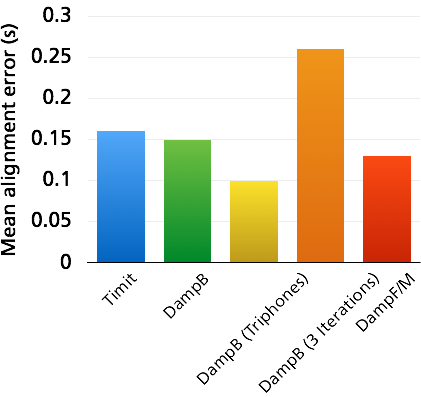
\includegraphics[width=.4\textwidth]{images/res_alignment.png}
		\caption{Mean alignment error in seconds on the \textit{ACAP} data set. \textit{Timit} shows the result for the same models used for aligning the new \textit{DAMP}-based data sets.}
		\label{fig:res_alignment}
	\end{center}
\end{figure}
The DNN models were trained to perform phoneme recognition. The results for those trained on \textit{TIMIT} are shown as the leftmost bars in figures \ref{fig:res_phonerec_acap} and \ref{fig:res_phonerec}. The first figure displays the results on the \textit{ACAP} data set. The phoneme error rate is $1.06$, the weighted phoneme error rate is $.8$. In the second figure, the same evaluation is performed on the \textit{DAMP} test data sets, with similar results: A phoneme error rate of $1.3$, and a weighted phoneme error rate of $.93$. This demonstrates that the performance of models trained on speech leaves room for improvement when used for phoneme recognition in singing.\\
It can be assumed that models trained on better-matching conditions (i.e. singing) would perform much better at this task. The problem with this approach lies in the lack of data sets that can be used for these purposes. In contrast with speech, no large corpora of phonetically annotated singing are available. In the following sections, several workarounds for this problem are tested.


\begin{figure*}
	\centering
	\begin{subfigure}[t]{0.3\textwidth}
		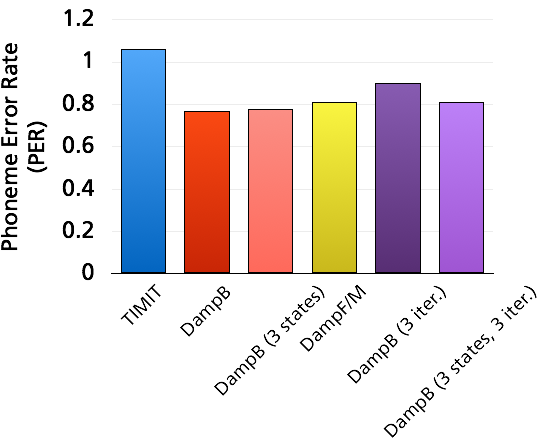
\includegraphics[width=\textwidth]{images/res_phonerec_acap.png}
		\caption{Phoneme error rate}
		
	\end{subfigure}%
	\begin{subfigure}[t]{0.3\textwidth}
		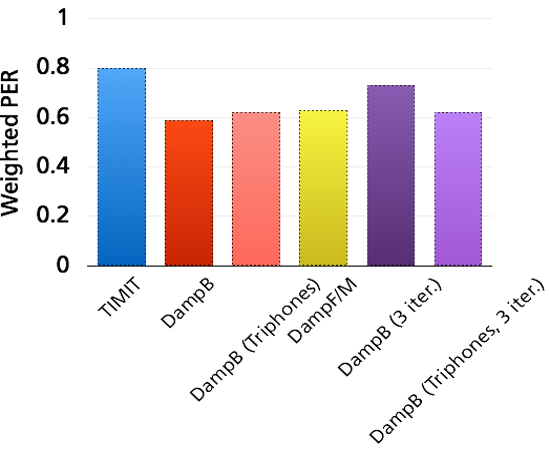
\includegraphics[width=\textwidth]{images/res_phonerec_acap_w.png}
		\caption{Weighted phoneme error rate}
	\end{subfigure}
	\caption{Mean phoneme recognition results on the \textit{ACAP} data set using acoustic models trained on \textit{Timit} and the new \textit{DAMP}-based data sets.}\label{fig:res_phonerec_acap}
\end{figure*}

\begin{figure*}
	\centering
	\begin{subfigure}[t]{0.3\textwidth}
		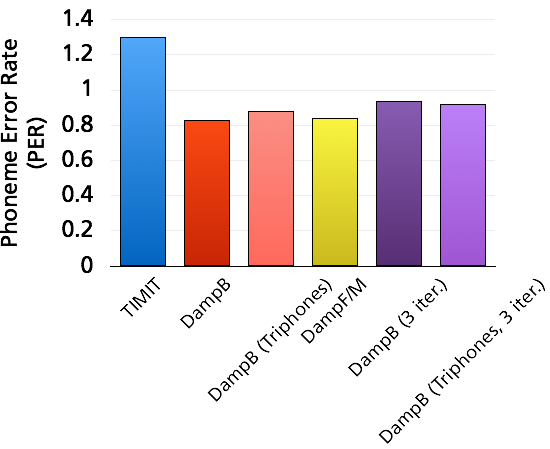
\includegraphics[width=\textwidth]{images/res_phonerec.png}
		\caption{Phoneme error rate}
		
	\end{subfigure}%
	\begin{subfigure}[t]{0.3\textwidth}
		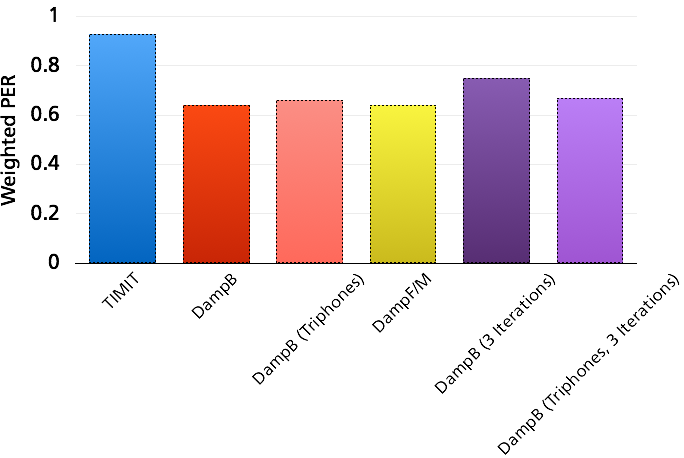
\includegraphics[width=\textwidth]{images/res_phonerec_w.png}
		\caption{Weighted phoneme error rate}
	\end{subfigure}
	\caption{Mean phoneme recognition results on the \textbf{DampTest} data sets using acoustic models trained on \textit{Timit} and the new \textit{DAMP}-based data sets.}\label{fig:res_phonerec}
\end{figure*}

\section{Phoneme recognition using models trained on ``songified" speech}
% time stretch, pitch shift
% variants
% dnn vs dbn??
% phonerec tested on: timit, acap
% todo: test on damp

When there is a scarcity of suitable training data, attempts are often made to generate such data artificially. For example, this is often done when models for noisy speech are required \cite{ntimit}\cite{aurora}. Inspired by this, one idea was making existing speech data sets more ``song-like'' and use these modified datasets to train models for phoneme recognition in singing. The \textit{TIMIT} corpus was once again used as a basis for this.\\

An overview of the approach is shown in figure \ref{fig:process_songify}. Five variants of the training part  \textit{TIMIT} were generated first. MFCC features were then extracted from these new datasets and used to train models.\\
Similarly, MFCCs are extracted from the \textit{TIMIT} Test set and from the \textit{ACAP} data set. The previously trained models are used to recognize phonemes on these test datasets. Viterbi decoding can then be used to generate phoneme sequences. Finally, the results are evaluated.
\setlength{\belowcaptionskip}{-0.4cm}
\begin{figure*}
 \begin{center}
                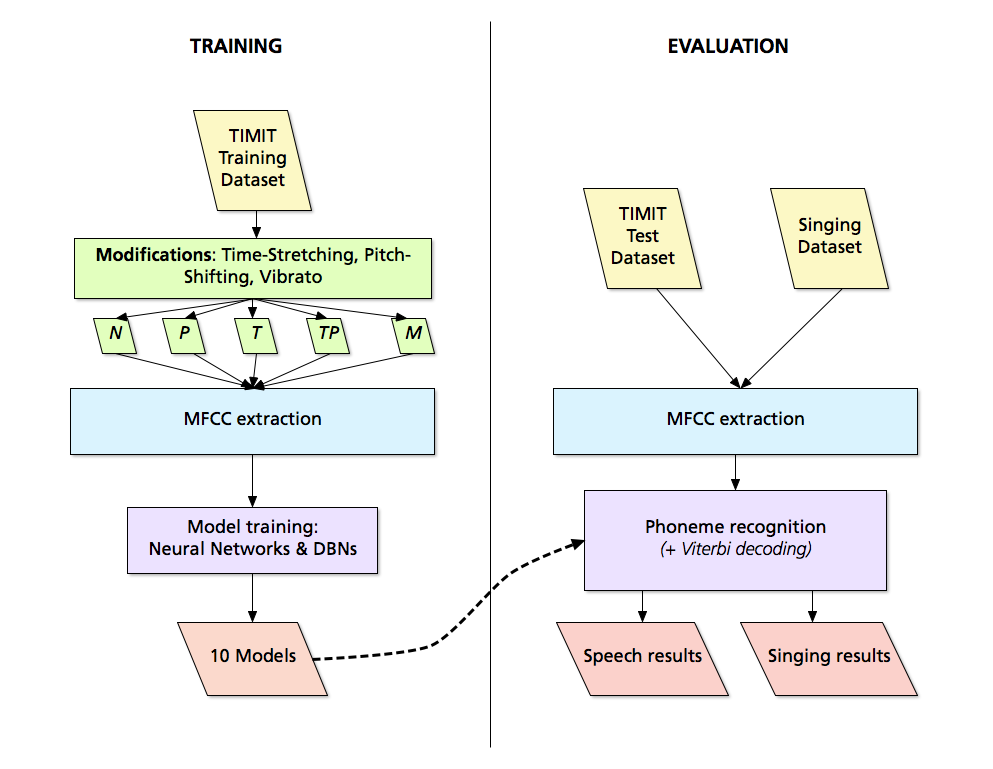
\includegraphics[width=0.7\textwidth]{images/process_songify.png}
                \caption{Overview of our phoneme recognition system}
                \label{fig:process_songify}
                 \end{center}
 \end{figure*}
 \setlength{\belowcaptionskip}{-0.1cm}
In order to make the training data more ``song-like'', several variants of this dataset were developed. Table \ref{tab:timit_variants} shows an overview over the five datasets generated from \textit{TIMIT} using three modifications. Dataset $N$ is the original \textit{TIMIT} training set. For dataset $P$, four of the eight blocks of \textit{TIMIT} were pitch-shifted. For dataset $T$, five blocks were time-stretched and vibrato was applied to two of them. In dataset $TP$, the same is done, except with additional pitch-shifting. Finally, dataset $M$ contains a mix of these modified blocks.\\
In detail, the modifications were performed in the following way:

\begin{description}
 \item[Time stretching] For time stretching, the phase vocoder from \cite{ellis_pvoc}, which is an implementation of the Flanagan/Dolson phase vocoder \cite{flanagan}\cite{dolson}, was used. This algorithm works by first performing a Short-Time Fourier Transform (STFT) on the signal and then resampling the frames to a different duration and performing the inverse Fourier transform.\\
 As demonstrated in section \ref{sec:speech_to_singing}, time variations in singing are mainly performed on vowels and are often much longer than in speech. Therefore, the \textit{TIMIT} annotations were used to only pick out the vowel segments from the utterances. They were modified randomly to a duration between $5$ and $100$ times the original duration and then re-inserted into the utterance. This effectively leads to more vowel frames in the training data, but since there is already a large amount of instances for each phoneme in the original training data, the effects of this imbalance should be negligible. 
 \item[Pitch shifting] To pitch-shift the signal, code from the freely available Matlab tool \textit{AutoTune Toy}\cite{autotunetoy}, which also implements a phase vocoder, was used. In this case, the fundamental frequency is first detected automatically. The signal is then stretched or expanded to obtain the new pitch and interpolated to retain the original duration.\\
 Using the \textit{TIMIT} annotations, utterances were split up into individual words, and then a pitch-shifted version of each word was generated and the results were concatenated. Pitches are randomly selected from a range between $60\%$ and $120\%$ of the original pitch.
 \item[Vibrato] The code for vibrato generation was also taken from \textit{AutoTune Toy}. It functions by generating a sine curve and using this as the trajectory for the pitch shifting algorithm mentioned above. A sine of amplitude $0.2$ and frequency $6 Hz$ was used.\\
 In singing, vibrato is commonly done on long sounds, which are usually vowels. Since spoken vowels are usually very short, vibrato cannot be perceived on them very well. Therefore, vibrato was only added when time stretching was also applied. Vibrato was then added to the extracted and stretched vowels.
\end{description}



\begin{table}
 \begin{center}
  \begin{tabular}{|c||c|c|c|c|c|}
  \hline
   & \textbf{N} & \textbf{P} &\textbf{T} &\textbf{TP} &\textbf{M} \\
  \hline
  DR1 & N & N & N & N & N  \\
  DR2 & N & N & N & N & N \\
  DR3 & N & N & N & N & P\\
  DR4 & N & N & T & TP & TV \\
  DR5 & N & P & T & TP & TPV \\
  DR6 & N & P & T & TP & TV \\
  DR7 & N & P & TV & TPV & P \\
  DR8 & N & P & TV & TPV & TPV \\
  \hline
 \end{tabular}
\end{center}
 \caption{The five TIMIT variants that were used for training (rows are TIMIT blocks, columns are the five datasets).
  Symbols: N - Unmodified; P - Pitch-shifted; T - Time-stretched; V - Vibrato}
 \label{tab:timit_variants}
\end{table}



\section{Phoneme recognition on synthesized singing}
% sinsy; female only
% dnn
%phonerec tested on:
% matched set, acap, dampf
%problem: correct instead of w_per!!

\section{Phoneme recognition using models trained on a-capella singing} \label{sec:phonerec_acap}
%how created?
% dnn
%phonerec tested on:
% acap, dampf/m
%alignment tested on acap; also: hmms!!

\subsection{Corpus construction}

%pre-existing; copy old paragraphs here
As a basis for our phonetically annotated data set, we used the \textit{DAMP} data set, which is freely available from Stanford University\footnote{\url{https://ccrma.stanford.edu/damp/}}\cite{phdthesis:jeffreysmith}. This data set contains more than 34,000 recordings of amateur singing of full songs (3 to 5 minutes duration) with no background music, which were obtained from the \textit{Smule Sing!} karaoke app. Each performance is labeled with metadata such as the gender of the singer, the region of origin, the song title, etc. The singers performed 301 different English language pop songs. The recordings have good sound quality with little background noise, but come from a lot of different recording conditions.


\begin{figure*}
 \begin{center}
                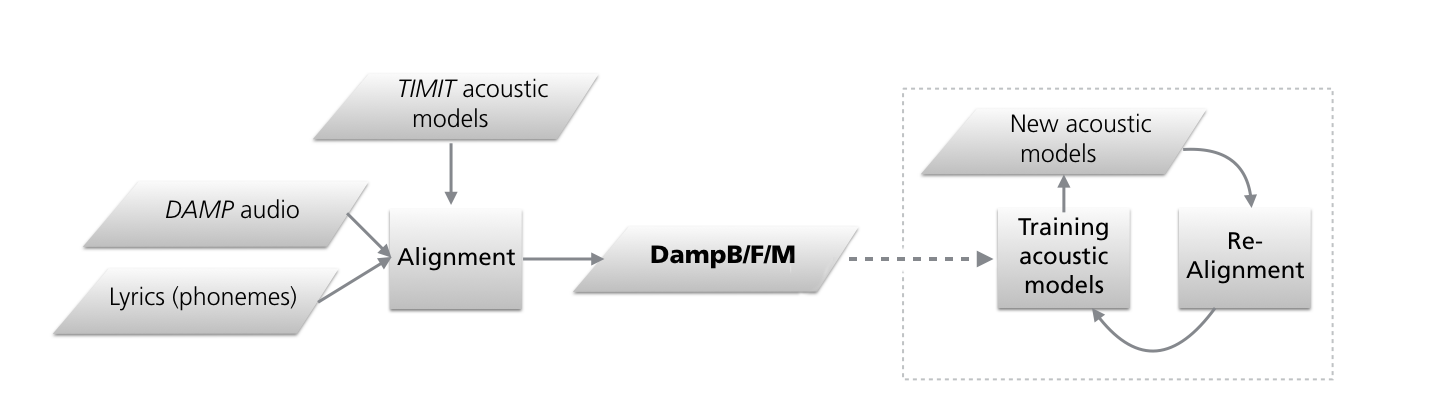
\includegraphics[width=.8\textwidth]{images/overview_bootstrap.png}
                \caption{An overview of the alignment process. The right-hand part represents the optional bootstrapping.}
                \label{fig:process}
                 \end{center}
 \end{figure*}
No lyrics annotations are available for this data set, but we obtained the textual lyrics from the \textit{Smule Sing!} website\footnote{\url{http://www.smule.com/songs}}.  All of them were English-language songs. These lyrics were mapped to their phonetic content using the CMU Pronouncing Dictionary\footnote{\url{http://www.speech.cs.cmu.edu/cgi-bin/cmudict}} with some manual additions of unusual words. This dictionary has a phoneme set of 39 phonemes.\\
We then performed an automatic alignment of these lyrics to the \textit{DAMP} audio.\\
As a basis, a monophonic HMM acoustic model trained on the \textit{Timit} speech corpus was used \cite{timit}. The model training and the alignment were done using the HTK framework \cite{htk}, which uses Viterbi alignment as its algorithm. MFCCs and their deltas and double-deltas were used as features. Alignment was performed on the word and phoneme levels. This is the same principle of so-called ``Forced Alignment" that is commonly used in Automatic Speech Recognition \cite{book:jurafsky} (although it is usually done on shorter utterances). \\
On top of this, we carried out several different alignment strategies:
\begin{description}
\item[Monophones vs. Triphones] We tested aligning both monophones (i.e. one state per phoneme) and triphones (i.e. three states per triphone modeling the start, middle, and end phases). Since \textit{Timit} only contains monophone annotations, this was done by first splitting the phoneme time frames evenly through three, and then re-training the \textit{Timit} acoustic model and re-aligning the data set (with the assumption that the transitions between the triphone states would be ``pulled'' to the correct times).  
\item[One-pass alignment vs. Bootstrapping] On top of a one-pass alignment using the Viterbi algorithm, we also investigated whether the acoustic models could be bootstrapped to improve the alignment. To clarify: We first performed the alignment on the \textbf{Damp} data sets using the \textit{Timit} models described above, then trained acoustic models on the resulting phoneme annotations. Then, those models were used to re-align the \textbf{Damp} data, which was again used to train another model. This was done over three iterations.\\
A modified version of the alignment algorithm was used for doing alignment with the models trained on the \textbf{Damp} data sets. This approach is based on doing Dynamic Time Warping on the generated phoneme posteriorgrams without punishing very long states. This is similar to the approach described in \cite{kruspe_lyrics_retrieval}.
\end{description}
A graphical overview of the alignment process is given in figure \ref{fig:process}.\\
Of course, errors cannot be avoided when doing automatic forced alignment. All in all, there were now four combinations of these strategies, which we compared. In section \ref{sec:validation}, we describe how this alignment procedure was validated and what strategies performed best.\\
Since there is usually a large number of recordings of the same song, we considered using this information to improve the alignment results, e.g. by averaging timestamps over the alignments of several recordings. We did not do this in this work because recordings tend to have different offsets from the beginning (i.e. silence in the beginning), and the singers also do not necessarily pronounce phonemes at the same time. This might be an avenue for future research, though.
\section{Validation}\label{sec:validation}
Validating the phoneme annotations created in this way is not trivial since there is no ground truth to base them on. We therefore used a two-pronged approach: We first tested the same alignment algorithm on a different, small, manually annotated data set. Second, we trained new acoustic models on the newly generated training data sets. We then performed phoneme recognition on the test data sets, and compared the results to the expected phoneme strings (which are known since we have the matching lyrics).
\subsection{Validation data}\label{subsec:validation_data}
For testing the alignment approach, we used a small data set of the vocal tracks of 15 pop songs, which were hand-annotated with phonemes and words. This data set was first presented in \cite{jens}. We call it \textit{ACAP}.
%Despite the small size, we provide results on this data set for comparison with our previous approaches, and because the ground truth annotations can be assumed to be correct (in contrast with the automatically generated annotations of the \textit{Damp}-based data sets).
%problem: no valid ground truth
\subsection{Alignment validation}
We first tested the same alignment approach that was used to create the new \textit{DAMP}-based data sets on the \textit{ACAP} data set. To recap: This approach employs models trained on the \textit{Timit} speech corpus, which are used for Viterbi alignment of the known phonemes to the singing. The result of this is then compared to the manual annotations by calculating the difference between each expected and predicted phoneme transition. 



We then tested various models trained on the new \textbf{DampB}, \textbf{DampF}, and \textbf{DampM} training data sets for the same task. The results are also shown in figure \ref{fig:res_alignment}.\\
Models trained on the monophonic alignments of \textbf{DampB} and \textbf{DampF/M} perform slightly better at this task with mean errors of $0.15$ and $0.13$ seconds respectively (for the gender-specific models, those values were only calculated for the songs of the matching gender in \textit{ACAP}). The triphone version of \textbf{DampB} performs even better, with a mean error of $0.1$. We believe this might be because dedicatedly training the model for the start and end parts of phonemes might make the alignment approach more accurate at finding start and end points.\\
Finally, we also tested the model trained on \textbf{DampB} over three iterations. This model performs much worse at this task. This might happen because errors in the original alignment of the phonemes may become amplified over these iterations.

\subsection{Validation of phoneme recognition}
To obtain a clearer picture of the quality of the new data sets, we also performed phoneme recognition experiments on both \textit{ACAP} and the \textbf{DampTest} corpora. This was possible even though there are no manual annotations for the \textbf{DampTest} sets because the expected phonemes are available from the textual lyrics. The phoneme error rate and the weighted phoneme error rate were used as evaluation measures (see \cite{kruspe_phonerec}).\\
The results for \textit{ACAP} are shown in figure \ref{fig:res_phonerec_acap}. In general, models trained on \textbf{DampB} performed much better at phoneme recognition than those trained on \textit{Timit}. Compared to these speech-based models, the phoneme error rate falls from $1.06$ to $0.77$, while the weighted phoneme error rate falls from $0.8$ to $0.59$. As can be seen from both evaluation measures, using triphone alignments instead of monophones does not improve the results in this case. This contrasts with the better alignment results. We think this might happen because more classes cause more confusion in the model, even though the triphone results were downmapped to monophones for calculating the evaluation measures.\\
As already seen in the alignment validation results, training models on \textbf{DampB} over three iterations actually degrades the result (``DampB (3)''). Again, we suspect that this happens because phoneme alignment errors become amplified in this way. Interestingly, this does not seem to happen for the triphone models, perhaps because the three classes per phoneme help to alleviate each other's errors.\\
The results for the same procedure on the \textbf{DampTest} sets are shown in figure \ref{fig:res_phonerec}. Results over \textbf{DampTestF} and \textbf{DampTestM} were averaged. This figure additionally shows the results for models trained on the gender-specific \textbf{DampF} and \textbf{DampM} data sets. These models were only tested on \textbf{DampTestF} and \textbf{DampTestM} respectively, and then the results were averaged.\\
We can observe the same general trend for these results: The phoneme error rate falls from $1.3$ to $0.87$ when compared to models trained on \textit{Timit}, with the weighted phoneme error rate decreasing from $0.93$ to $0.65$. Using triphones does not contribute to the result, and neither does the three-iteration bootstrapping process for training acoustic models. Interestingly, not even the gender-specific models improve the result. As already described in \cite{kruspe_phonerec}, this effect might occur because the range of pitch and expressions is much wider in singing than in speech, and therefore gender-specific models may not actually learn as much added helpful information.



\subsection{Error sources}
Of course, with an automatic alignment algorithm like this, errors cannot be avoided. To acquire a clearer picture of the reasons for the various misalignments, we had a closer look at the audio data where they occurred. Some sources of error repeatedly stuck out:
%\begin{compactdesc}
\begin{description}
 \item[Unclear enunciation]{Some singers pronounced words very unclearly, often focusing more on musical performance than on the lyrics.}
 \item[Accents]{Some singers sung with an accent, either their natural one or imitating the one used by the original singer of the song.}
 \item[Young children's voices]{Some recordings were performed by young children.}
 \item[Background music]{Some singers had the original song with the original singing running in the background.}
 \item[Speaking in breaks]{Some singers spoke in the musical breaks.}
 \item[Problems in audio quality]{Some recordings had qualitative problems, especially loudness clipping.}
%\end{compactdesc}
\end{description}
For most of these issues, more robust phoneme recognizers would be helpful. For others, the algorithm could be adapted to be robust to extraneous recognized phonemes (particularly for the speaking problem). If possible, a thorough manual check of the data would be very helpful as well.



\section{Conclusion}
